%----------------------------------------------------------------------------------------
%	PACKAGES AND OTHER DOCUMENT CONFIGURATIONS
%---------------------------------------------------------------------------------------

% if you're here it means you were interested enough in me try and find our a little more. Why don't you skip the digging and go right to the source?


\documentclass[
	10pt, % Default font size, can be between 8pt and 12pt
]{FreemanCV}


% Handle images:
\graphicspath{{./images/}}


\columnratio{0.60, 0.40} % Widths of the two columns, specified here as a ratio summing to 1 to correspond to percentages; adjust as needed for your content 

% Headers and footers can be added with the following commands: \lhead{}, \rhead{}, \lfoot{} and \rfoot{}
% Example right footer:
%\rfoot{\textcolor{headings}{\sffamily Last update: \today. Typeset with Xe\LaTeX}}

%----------------------------------------------------------------------------------------

\begin{document}

\begin{paracol}{2} % Begin two-column mode

%----------------------------------------------------------------------------------------
%	YOUR NAME AND CURRICULUM VITAE TITLE
%----------------------------------------------------------------------------------------

\parbox[][0.05\textheight][c]{\linewidth}{ % Box to hold your name and CV title; change the fixed height as needed to match the colored box to the right
	\centering % Horizontally center text
	% \hfill
	{\sffamily\fontsize{35}{60}\selectfont Josh \textbf{Booth}}
	% {\sffamily\HUGE Josh \textbf{Booth}} % Your name
}

\switchcolumn % Switch to the second (right) column

%----------------------------------------------------------------------------------------
%	COLORED CONTACT DETAILS BOX
%----------------------------------------------------------------------------------------

\parbox[top][0.1\textheight][c]{\linewidth}{ % Box to hold the colored box; change the fixed height as needed to match the box to the left
	\colorbox{shade}{ % Create colored box and specify background color
		\begin{supertabular}{@{\hspace{3pt}} p{0.05\linewidth} | p{0.775\linewidth}} % Start a table with two columns, the table will ensure everything is aligned
			\raisebox{-1pt}{\faPhone} & (717) 494-6466 \\ % Phone number
			\raisebox{-1pt}{\small\faEnvelope} & \href{mailto:boothjmail@gmail.com}{boothjmail@gmail.com} \\ % Email address
			%\raisebox{-1pt}{\small\faLink} & \href{https://joshbooth.us}{joshbooth.us} \\ % Website
			\raisebox{-1pt}{\faHome} & Chandler, AZ \\ % Address
			%\raisebox{-1pt}{\faGithub} & \href{https://github.com/username}{https://github.com/username} \\ % GitHub profile
			\raisebox{-1pt}{\faLinkedinSquare} & \href{https://www.linkedin.com/in/joshua-f-booth/}{Linkedin} \\ % LinkedIn profile
			% See fontawesome.pdf in the Fonts folder for all icons you can use
		\end{supertabular}
	}
	\vfill % Push content to the top of the box
}
\end{paracol}
		

%----------------------------------------------------------------------------------------
%	WORK EXPERIENCE
%----------------------------------------------------------------------------------------
\vspace{-35pt}

\section{Work Experience}

% Each job is added with a \jobentry command. Below is an empty one to use as a template:

%\jobentry
%	{} % Duration
%	{} % FT/PT (full time or part time)
%	{} % Employer
%	{} % Job title
%	{} % Description

% All 5 parameters must be supplied but any can be empty if you don't need them

%------------------------------------------------

\jobentry
	{Current, from Jun 2022} % Duration
	{FT} % FT/PT (full time or part time)
	{Microchip Technology} % Employer
	{Applications/Marketing Engineer} % Job title
	{ % Description
		\item Wrote production-quality embedded C code for customers to use as a reference when creating their own designs.
		\item Developed various demos on PIC and AVR microcontrollers for new products (see DMX Light Show, The Cold Plate). This included writing and documenting code and test conditions as well as completing design documents and flowcharts for the published demo.
		\item Created and documented example libraries for abstracted use in collaboration with a local/global team.
		\item Executed project analysis to synchronize deliverables to management. This included identifying project purposes, documenting key deliverables, code hooks, and team responsibilities as well as updating Airtable with weekly updates.
		\item Designed PCBs and structural enclosures for the demos.
		\item Led an analytics initiative that helped improve video retention and click rate for marketing campaigns.
	} 

% ---------------------------------------------

\jobentry
	{Sep 2016, Jun 2022} % Duration
	{FT/PT} % FT/PT (full time or part time)
	{Booth Oil and Gas LLC.} % Employer
	{Prototype Engineer} % Job title
	{ % Description
		\item Designed and manufactured prototypes for novel business problems (see 3D PEEK Printer, AI-Driven Security System).
		\item Offered technical expertise for project planning, cost estimation, and feasibility studies.
		\item Communicated with the client to manage their expectations and incorporate or remove features as their needs changed.
	}
	

%------------------------------------------------

\jobentry
	{Jun 2017 - Jan 2022} % Duration
	{FT/PT} % FT/PT (full time or part time)
	{United States Naval Research Laboratory} % Employer
	{Electrical Engineer} % Job title
	{ % Description
		\item Detecting and classifying objects in satellite imagery using TFLearn and pachyderm for rapid machine learning model prototyping.
		\item Recovered RF communications lost to noise by augmenting message-passing algorithms with machine learning.
		\item Identified promotor sequences in DNA to speed up genome sequence identification (BRNN w/ LSTM cells.)
	} 


%----------------------------------------------------------------------------------------
%	ENGINEERING PROJECTS
%----------------------------------------------------------------------------------------

\vspace*{-10pt}
\section{Embedded Development Projects}
\columnratio{0.5, 0.5}
\setlength{\columnsep}{10pt}

\begin{paracol}{2} % Begin four-column mode

% The Cold Plate
\vspace*{-10pt}
\leavevmode \subsection{\href{https://github.com/microchip-pic-avr-examples/pic16f17146-cold-plate-mplab-mcc}{The Cold Plate \linkcolor\scriptsize\faLink}
\hfill
\textsc{\footnotesize{(Embedded C, analog \& power design)}}}

\setlength\intextsep{0pt} % image in vertical relation to subsection title
\begin{wrapfigure}[7]{r}{0pt} % # of narrow lines, right top alignment, image L/R adjustment
	\hspace*{-5pt} % how close horizontal text can be
    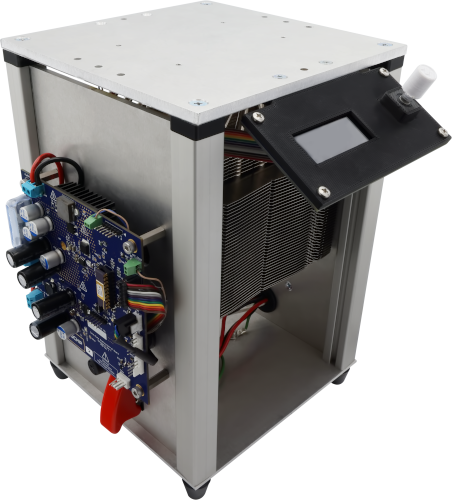
\includegraphics[width=70pt]{cold_plate} %Z how large image is
\end{wrapfigure}

A reference design showing the most efficient way to perform common microcontroller tasks on a PIC16
such as temperature measurement, fan control, current monitoring, and UI control;
all wrapped up into an engaging demo.\\

This project demonstrates my ability to develop clean code and documentation as well as working within a team.\\
It has become Microchip's most copied code repository.


% DMX Light Show
\vspace*{-10pt} % title's anchor box
\leavevmode\subsection{DMX Light Show
\hfill
\textsc{\footnotesize{(Embedded C, analog \& power design)}}}

\setlength\intextsep{-5pt} % image in vertical relation to subsection title
\begin{wrapfigure}[7]{r}{0pt} % # of narrow lines, right top alignment, image L/R adjustment
	\hspace*{-5pt} % how close horizontal text can be
    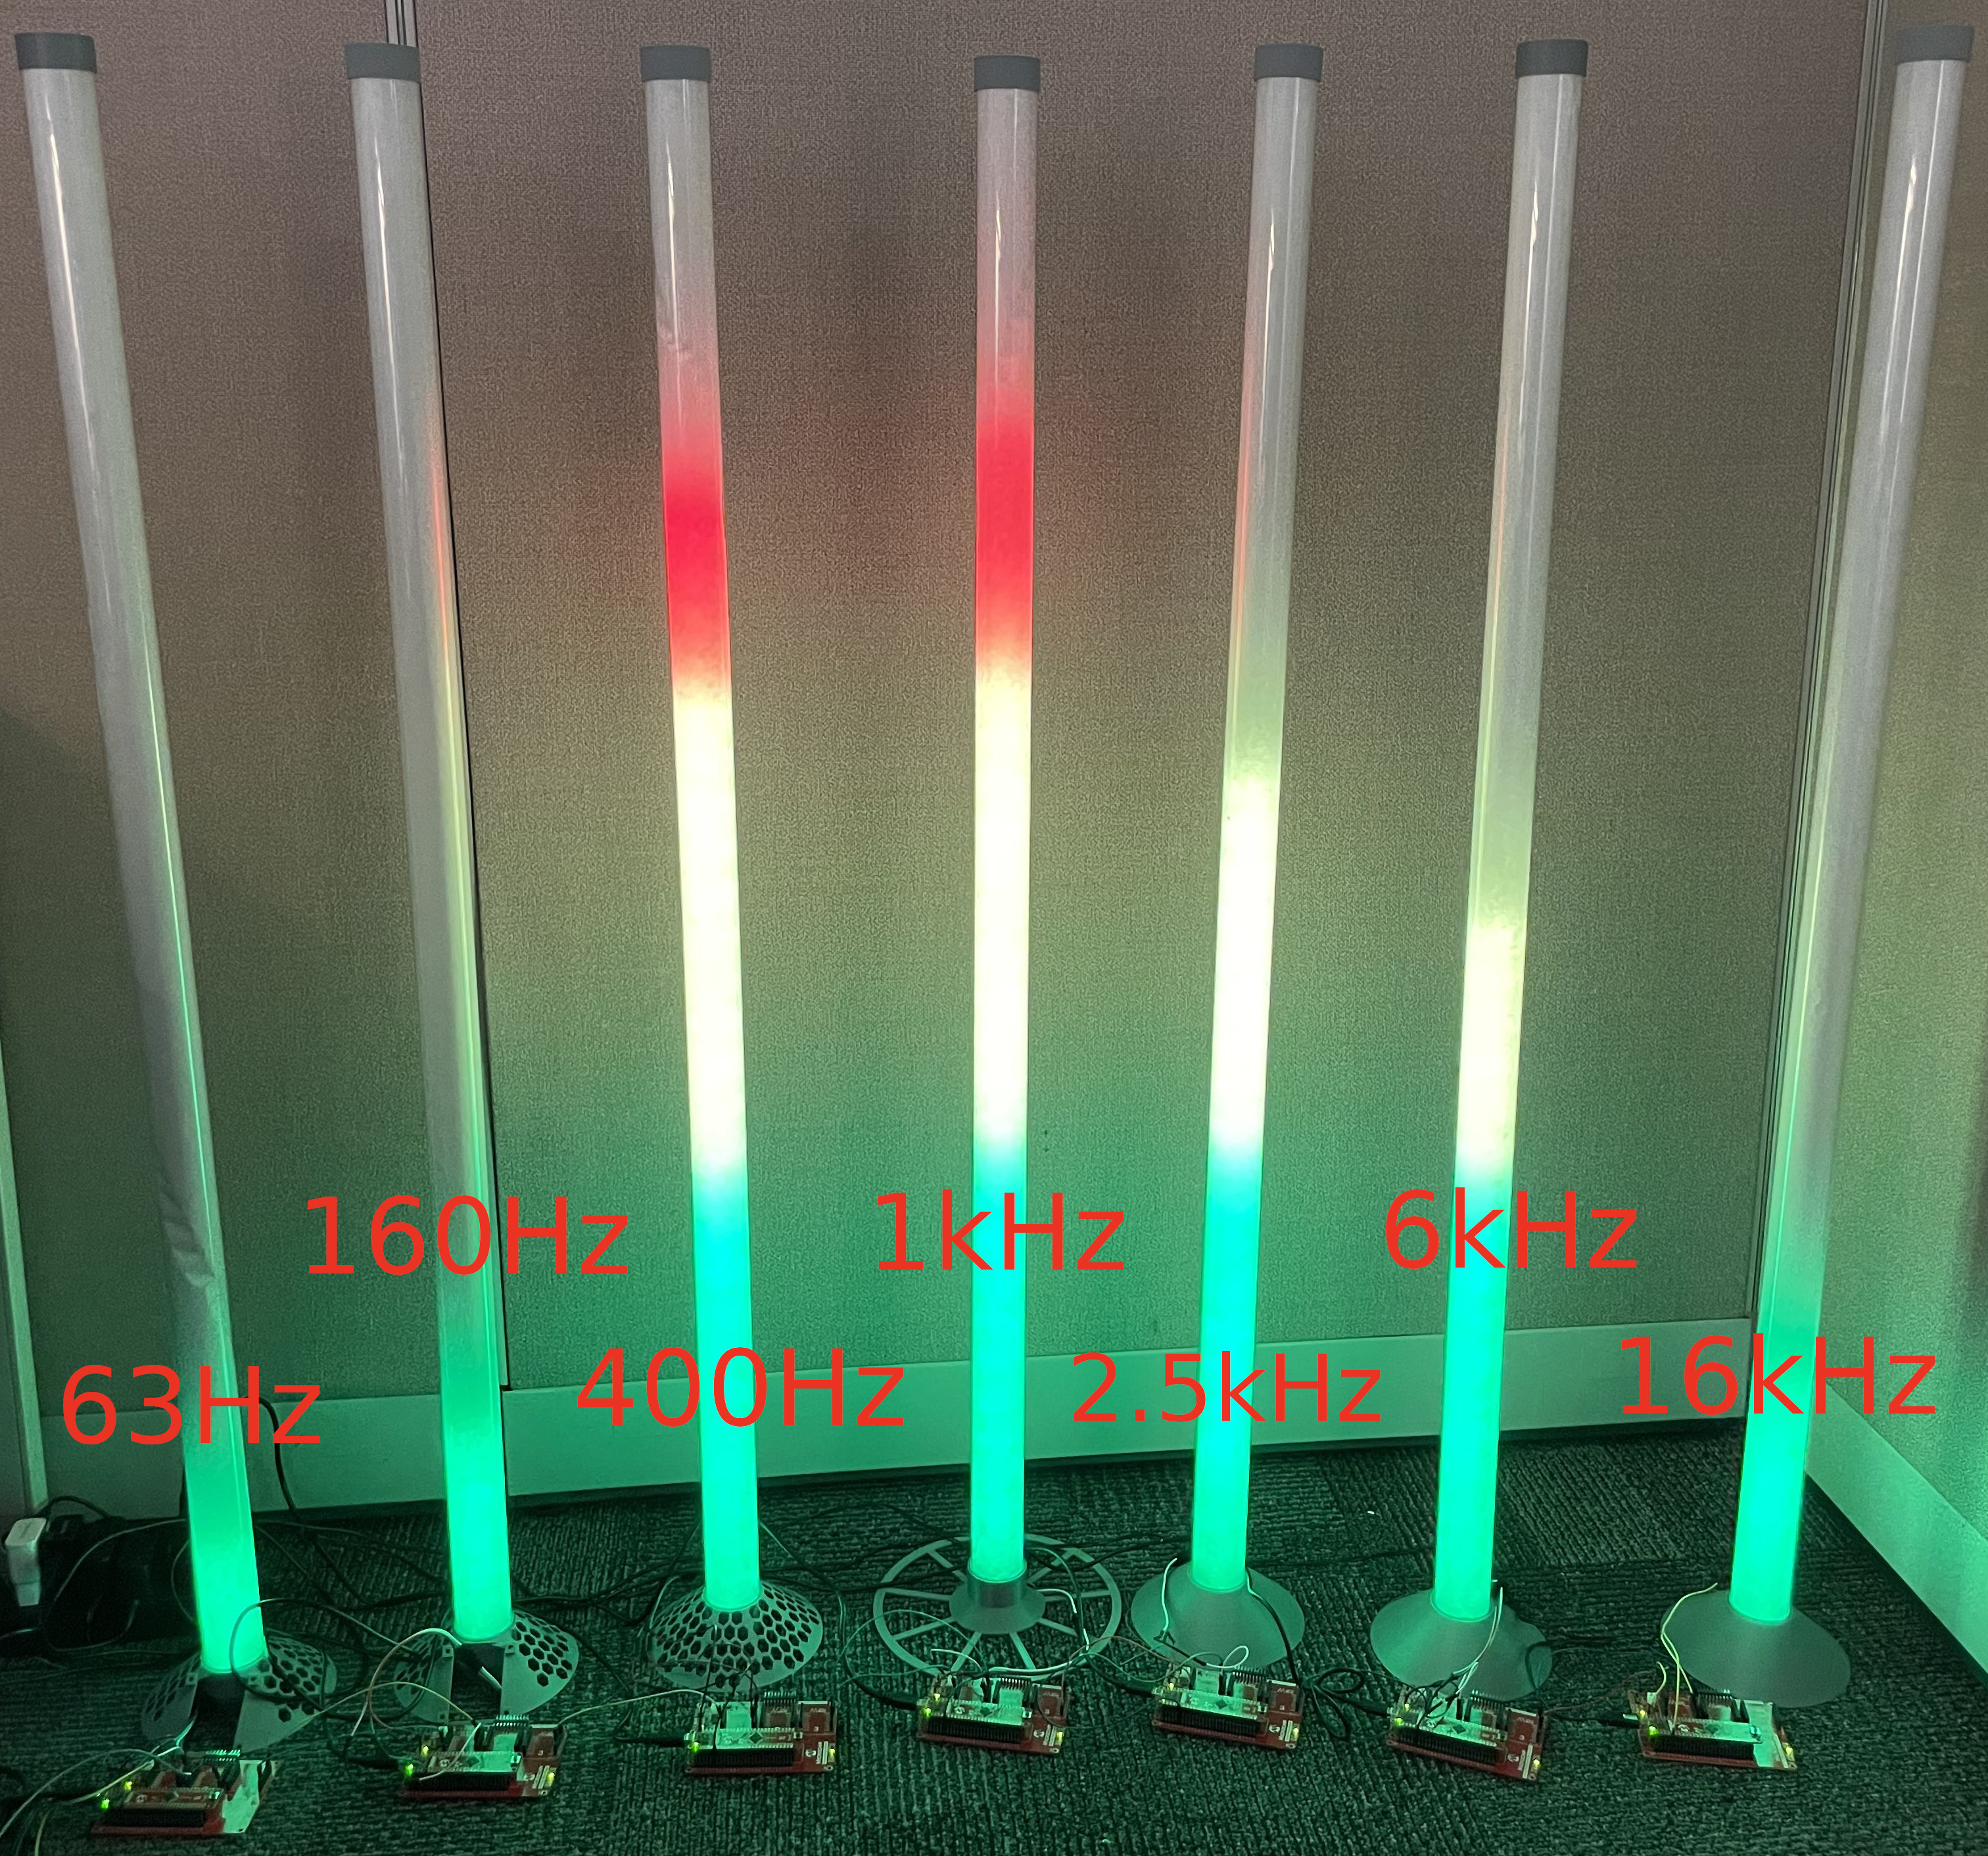
\includegraphics[width=90pt]{dmx} %Z how large image is
\end{wrapfigure}

A real-time audio processing light show integrating audio filtering, DMX, DMA, PoE, and a hardware-encoded WS2812 driver; each node using a PIC18Q71 MCU. Utilizing the devices' CIPs, nearly no processing occurs on the CPU.\\

Written C drivers for this project include UART, DMA, DMX, PWM, SPI, CLC, OP-AMP, and ADC configurations.

\switchcolumn

% 3D PEEK Printer
\vspace*{-10pt}
\leavevmode \subsection{\href{https://github.com/jfcbooth/3dpp}{3D PEEK Printer \linkcolor\scriptsize\faLink}
\hfill
\textsc{\footnotesize{(Embedded C, Python, analog \& power design)}}}

\setlength\intextsep{-5pt} % image in relation to subsection title
\begin{wrapfigure}[9]{r}{0pt} % # of narrow lines, right top alignment, image L/R adjustment
	\hspace*{-5pt} % how close horizontal text can be
    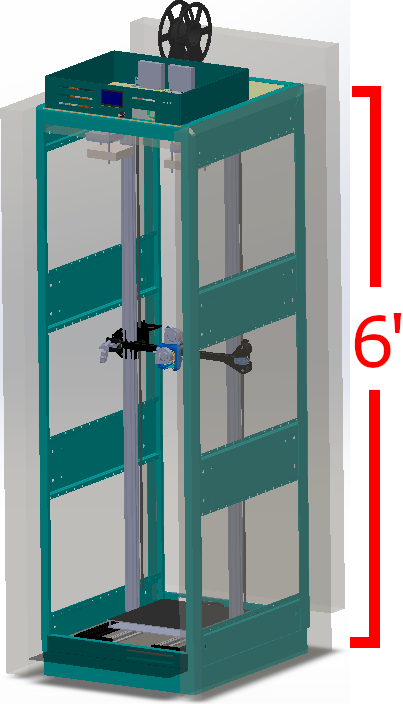
\includegraphics[width=60pt]{printer} %Z how large image is
\end{wrapfigure}

Designed and built a large-scale 3D printer capable of printing PEEK for biofuel refinement.\\

An STM32 MCU running Klipper and a Raspberry Pi running custom Python controlled the printer.
Involved in the development was designing the kinematic system, thermal dynamics, and software to safely control its operation
while dealing with hazardous temperatures and voltages.


% AI Driven Security system
\vspace*{0pt}
\leavevmode \subsection{\href{https://github.com/jfcbooth/security_system}{AI-Driven Security System \linkcolor\scriptsize\faLink}
\hfill
\textsc{\footnotesize{(Python, Bash, Machine Learning)}}}

\setlength\intextsep{0pt} % image in relation to subsection title
\begin{wrapfigure}[8]{r}{0pt} % # of narrow lines, right top alignment, image L/R adjustment
	\hspace*{-5pt} % how close horizontal text can be
    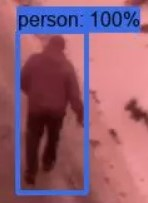
\includegraphics[width=60pt]{security_system} %Z how large image is
\end{wrapfigure}

A solar-powered security system that gives real-time alerts with a classified video anytime a human, vehicle, or large animal is spotted
on the property.\\

Custom python and bash programs handled data transfer throughout the mesh network and into/out of the neural network.


\end{paracol}


% Entry 4 - image on right
% Hadley Electric Stand

% \setlength\intextsep{7pt} % image in relation to subsection title
% \begin{wrapfigure}[8]{rt}{25pt} % # of narrow lines, right top alignment, image L/R adjustment
% 	\hspace*{-23pt} % how close horizontal text can be
%     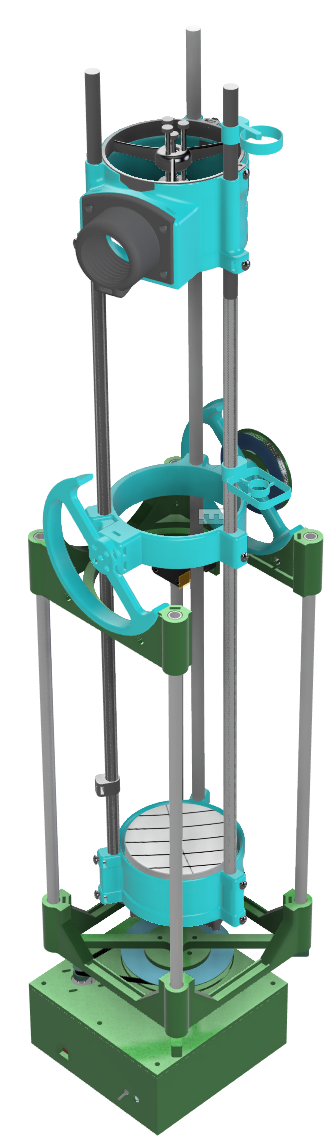
\includegraphics[width=45pt]{hadley_electric_stand2} %Z how large image is
% \end{wrapfigure}

% \vspace*{-10pt} % move title's anchor box up closer to title
% \leavevmode\subsection{\href{https://github.com/jfcbooth/hadley_electric_stand}{Hadley Electric Stand - Open Source Project\scriptsize\faLink}}

% Hadley is a \$150 telescope, capabable of giving 
	

% 	%------------------------------------------------

% \end{supertabular}
% % END EDUCATION

%----------------------------------------------------------------------------------------
%	PUBLICATIONS
%----------------------------------------------------------------------------------------

\section{Publications}

%------------------------------------------------

\begin{supertabular}{p{0.05\linewidth} p{0.88\linewidth}} % Start a table with two columns, the table will ensure everything is aligned
	
	%------------------------------------------------
	2023 & \href{
	https://ww1.microchip.com/downloads/aemDocuments/documents/MCU08/ApplicationNotes/ApplicationNotes/AN4889-Using-CIPs-To-Implement-Peltier-Plate-DS00004889.pdf
	}{
	App. Note 4889: Using Core Independent Peripherals (CIPs) to Implement a Peltier Cooled Metal Plate
	\linkcolor\scriptsize\faLink} \\
	%------------------------------------------------
	2023 & \href{
	https://www.embedded.com/reducing-bom-cost-in-embedded-systems-using-advanced-mcu-peripherals/
	}{
	Embedded.com - Reducing BOM cost in embedded systems using advanced MCU peripherals
	\linkcolor\scriptsize\faLink} \\
	%------------------------------------------------
	% 2023 & \href{
	% 	https://gateway.on24.com/wcc/eh/3685667/lp/4156150/learn-the-smart-way-to-use-on-chip-hardware-accessories-to-replace-discrete-components
	% }{
	% Webinar - Learn the Smart Way to Use On-Chip Hardware Accessories to Replace Discrete Components 
	% \scriptsize\faLink} \\
	%------------------------------------------------
	2018 & \href{
	http://joshbooth.us/wp-content/uploads/2023/08/Machine-Learning-in-Radio-Frequency-Communications.pdf
	}{
	Machine Learning in Radio Frequency Communications
	\linkcolor\scriptsize\faLink} \\
	%------------------------------------------------
	2017 & \href{
	http://joshbooth.us/wp-content/uploads/2023/08/poster_SBME_promoter_predictions.pdf
	}{
	Prediction of Bacterial Promoter Sequences using Machine Learning
	\linkcolor\scriptsize\faLink} \\
	%------------------------------------------------
	
\end{supertabular}

\medskip % Extra whitespace before the next section

%----------------------------------------------------------------------------------------
%----------------------------------------------------------------------------------------
%----------------------------------------------------------------------------------------

% END OF COLUMN 1

%----------------------------------------------------------------------------------------
%----------------------------------------------------------------------------------------
%----------------------------------------------------------------------------------------


\columnratio{0.45, 0.65}
\begin{paracol}{2}

%----------------------------------------------------------------------------------------
% EDUCATION
\section{Education} 
%----------------------------------------------------------------------------------------

% Each qualification entry is added with a \qualificationentry command. Below is an empty one to use as a template:
%------------------------------------------------

\begin{supertabular}{l l} % Start a table with two columns, the table will ensure everything is aligned

	%------------------------------------------------
	
	% \textsc{#1} & 
	\textbf{B.S. in Computer Engineering; Mathematics minor}\\ % Duration and degree
	\small\textsc{Summa Cum Laude; 3.98 GPA; CMPE 322/120 SI; Class of 2022}\\ % Honors, achievements or distinctions (e.g. first class honors)
	\textit{Shippensburg University of Pennsylvania}\\ % Institution
	
	%------------------------------------------------

\end{supertabular}
% END EDUCATION

\switchcolumn

\section{Core Competancies}

% \hangindent=10pt
% \hangafter=1
\begin{itemize}[leftmargin=10pt]
	\itemsep0pt
	\item \textbf{Technical:} C, Python, Linux, Marlin, Bash, Embedded Development,\\
	\hspace*{45pt}C++, Digital Circuit Design, CAD Design, Robotics
	\item \textbf{Software:} Git, Sourcetree, Fusion 360, KiCAD, Eagle, MPLAB X, XC8
	% \item \textbf{Other:} System Administration, \\Embedded Communications Protocols (I2C, SPI, DMX, UART, CAN), IT Professional
\end{itemize}
 % Description


%----------------------------------------------------------------------------------------
%	AWARDS
%----------------------------------------------------------------------------------------

% \section{Certifications/Awards}

% % This section is laid out using a table. A \tableentry command adds lines with the following parameters:

% %\tableentry{Heading}{Content}{spaceafter}
% % All 3 parameters must be supplied but any can be empty if you don't need them
% % A "spaceafter" value in the third parameter will add some vertical space -- this is to be used between headings, leave it empty for no extra space

% %------------------------------------------------

% \begin{supertabular}{r l} % Start a table with two columns, the table will ensure everything is aligned
	
% 	%------------------------------------------------
	
% 	\tableentry{2020}{Secret Security Clearance (inactive Mar 2022)}
% 	\tableentry{2018}{Eagle Scout}
% 	\tableentry{2017}{CompTia A+ Certified}
	
% 	%------------------------------------------------
	
% \end{supertabular}

\end{paracol}
%----------------------------------------------------------------------------------------
%	COMPUTER SKILLS
%----------------------------------------------------------------------------------------

% \section{Misc. Skills} 

% % This section is laid out using a table. A \tableentry command adds lines with the following parameters:

% %\tableentry{Heading}{Content}{spaceafter}
% % All 3 parameters must be supplied but any can be empty if you don't need them
% % A "spaceafter" value in the third parameter will add some vertical space -- this is to be used between headings, leave it empty for no extra space

% %------------------------------------------------

% \begin{supertabular}{r l} % Start a table with two columns, the table will ensure everything is aligned
	
% 	%------------------------------------------------
	
% 	\tableentry{Beginner}{Java, MS DOS}{spaceafter}
	
% 	%------------------------------------------------
	
% 	\tableentry{Intermediate}{Javascript, Python, HTML, CSS,}{}
% 	\tableentry{}{Microsoft Windows}{}
% 	\tableentry{}{Computer Hardware \& Support}{spaceafter}
	
% 	%------------------------------------------------
	
% 	\tableentry{Expert}{Perl, Unix, \LaTeX}{spaceafter}
	
% 	%------------------------------------------------
	
% \end{supertabular}

%----------------------------------------------------------------------------------------
%	COMMUNICATION SKILLS
%----------------------------------------------------------------------------------------

% \section{Communication Skills}

% % This section is laid out using a table. A \tableentry command adds lines with the following parameters:

% %\tableentry{Heading}{Content}{spaceafter}
% % All 3 parameters must be supplied but any can be empty if you don't need them
% % A "spaceafter" value in the third parameter will add some vertical space -- this is to be used between headings, leave it empty for no extra space

% %------------------------------------------------

% \begin{supertabular}{r l} % Start a table with two columns, the table will ensure everything is aligned
	
% 	%------------------------------------------------
	
% 	\tableentry{Conferences}{Oral Presentation at the Annual MIT}{}
% 	\tableentry{}{Theoretical Physics Conference -- 1987}{spaceafter}
	
% 	%------------------------------------------------
	
% 	\tableentry{Posters}{Poster at the Meeting of the American}{}
% 	\tableentry{}{Physical Society -- 1985}{spaceafter}
	
% 	%------------------------------------------------
	
% \end{supertabular}

%----------------------------------------------------------------------------------------

% \end{paracol} % End two-column mode

% \section{Core Competancies}
% \begin{itemize}
% 	\itemsep 0pt
% 	\item \textbf{Technical:} C, Python, Linux, Marlin, Embedded Development, Digital Circuit Design, 3D CAD Design, Data Analytics
% 	\item \textbf{Software:} Git, Fusion 360, KiCAD, Eagle, Sourcetree, MPLAB X, XC8, Bash, FreeCAD
% 	\item \textbf{Other:} System Administration, Embedded Communications Protocols (I2C, SPI, DMX, UART, CAN), IT Professional
% \end{itemize}
% %----------------------------------------------------------------------------------------

\end{document}
